% ============================================================================
% CSCE 763: Digital Image Processing - Homework 1
% ============================================================================

\documentclass[12pt]{article}

% ============================================================================
% PACKAGE IMPORTS
% ============================================================================
\usepackage{amsmath}
\usepackage{graphicx}
\usepackage{amssymb}
\usepackage{tikz}
\usepackage[margin=1in]{geometry}
\usepackage{setspace}
\usepackage{xcolor}
\usepackage{enumitem}
\usepackage{tcolorbox}
\usepackage{fancyhdr}
% lastpage removed - not available
\usepackage{booktabs}
\usepackage{array}
\usepackage{colortbl}
\usepackage{float}

% ============================================================================
% HEADER AND FOOTER SETUP
% ============================================================================
\pagestyle{fancy}
\setlength{\headheight}{14.5pt}
\fancyhf{}

\fancyhead[L]{Page \thepage}
\fancyhead[C]{CSCE 763}
\fancyhead[R]{JC Vaught}

\renewcommand{\headrulewidth}{0pt}

% ============================================================================
% TIKZ LIBRARIES
% ============================================================================
\usetikzlibrary{shapes.geometric, arrows.meta, positioning, patterns}

% --- USC Brand Colors ---
\definecolor{USC_Garnet}{HTML}{73000A}
\definecolor{USC_Sandstorm}{HTML}{FFF2E3}
\definecolor{USC_Black90}{HTML}{363636}
\definecolor{USC_Black70}{HTML}{5C5C5C}
\definecolor{USC_Black50}{HTML}{A2A2A2}
\definecolor{USC_Black10}{HTML}{ECECEC}
\definecolor{USC_Honeycomb}{HTML}{65780B}
\definecolor{USC_Atlantic}{HTML}{466A9F}
\definecolor{USC_Congaree}{HTML}{1F414D}
\definecolor{USC_Rose}{HTML}{CC2E40}
\definecolor{outputbg}{RGB}{245,245,245}

% ============================================================================
% CUSTOM COLORED BOXES
% ============================================================================
\newtcolorbox{stepbox}[1][Step]{
  colback=white,
  colframe=USC_Garnet,
  fonttitle=\bfseries,
  title=#1,
  sharp corners,
  colbacktitle=USC_Garnet,
  coltitle=white,
}

\newtcolorbox{resultsbox}{
  colback=white,
  colframe=USC_Honeycomb,
  fonttitle=\bfseries,
  title=Results,
  sharp corners,
  colbacktitle=USC_Honeycomb,
  coltitle=white,
}

% ============================================================================
% CUSTOM QUESTION AND PART COMMANDS
% ============================================================================
\newcommand{\question}[1]{%
  \clearpage
  \vspace{0.5cm}
  {\noindent\normalsize \textbf{#1}}
  \vspace{0.2cm}
  \hrule
  \vspace{0.1cm}
  \hrule
  \vspace{0.3cm}
}

\newcommand{\questionpart}[1]{%
  \clearpage
  \vspace{0.5cm}
  {\noindent\normalsize \textbf{#1}}
  \vspace{0.2cm}
  \hrule
  \vspace{0.1cm}
  \hrule
  \vspace{0.3cm}
}

% Graphics path
\graphicspath{{figures/}}

% ============================================================================
% DOCUMENT INFORMATION
% ============================================================================

\title{CSCE 763: Digital Image Processing \\ Homework \#1}
\author{Instructor: Spring 2026 \\ University of South Carolina \\ \textit{Solutions by: JC Vaught}}
\date{Due: 1:15 pm EST, Tuesday, Feb 3}

% ============================================================================
% BEGIN DOCUMENT
% ============================================================================

\begin{document}

\maketitle
\setlength{\parindent}{0pt}

\setlist[enumerate,1]{label=\arabic*.}
\setlist[enumerate,2]{label=(\alph*)}

% ============================================================================
% TABLE OF CONTENTS
% ============================================================================

\begin{center}
\begin{tcolorbox}[colback=white, colframe=gray!50!black, colbacktitle=gray!20!white,
                  coltitle=black, sharp corners, boxrule=1pt,
                  title=\Large\bfseries Table of Contents]
\begin{tabular}{p{0.82\textwidth}r}
\textbf{Problem 1: Smallest Discernible Dot (25 pts)} \dotfill & \textbf{\pageref{quest:1}} \\[0.3em]
\textbf{Problem 2: Adjacency of Image Subsets (25 pts)} & \\
\quad Part (a): 4-adjacency \dotfill & \textbf{\pageref{quest:2}} \\
\quad Part (b): 8-adjacency \dotfill & \textbf{\pageref{quest:2}} \\
\quad Part (c): m-adjacency \dotfill & \textbf{\pageref{quest:2}} \\[0.3em]
\textbf{Problem 3: Shortest Paths (25 pts)} & \\
\quad Part (a): $V = \{0, 1\}$ \dotfill & \textbf{\pageref{quest:3}} \\
\quad Part (b): $V = \{1, 2\}$ \dotfill & \textbf{\pageref{quest:3}} \\[0.3em]
\textbf{Problem 4: Set Expressions (25 pts)} \dotfill & \textbf{\pageref{quest:4}} \\
\end{tabular}
\vspace{0.2cm}
\end{tcolorbox}
\end{center}

\vspace{0.5cm}

% ============================================================================
% PROBLEM 1: Smallest Discernible Dot
% ============================================================================

\question{Problem 1: Smallest Discernible Dot (25 pts)}\label{quest:1}

Thinking purely in geometric terms, estimate the diameter of the smallest printed dot that the eye can discern if the page on which the dot is printed is 0.5\,m away from the eyes.

\textbf{Assumptions:}
\begin{enumerate}
    \item The distance between the center of the lens and the retina along the visual axis is 14\,mm.
    \item The visual system ceases to detect the dot when the image of the dot on the fovea becomes smaller than the diameter of one receptor (cone) in that area of the retina.
    \item The fovea can be modeled as a square array of dimensions $1.5\,\text{mm} \times 1.5\,\text{mm}$, and the cones (about 337{,}000 in total) and spaces between the cones are distributed uniformly throughout this array.
\end{enumerate}

\vspace{0.3cm}

\begin{stepbox}[Step 1: Determine the Diameter of a Single Cone]
The fovea is a $1.5\,\text{mm} \times 1.5\,\text{mm}$ square with 337{,}000 cones uniformly distributed. Modeling as a square grid, the number of cones per side is:
\[
n = \sqrt{337{,}000} \approx 580.5
\]

The center-to-center spacing (cone diameter including gaps) is:
\[
d_{\text{cone}} = \frac{1.5\,\text{mm}}{580.5} \approx 0.00258\,\text{mm} = 2.58\,\mu\text{m}
\]
\end{stepbox}

\begin{stepbox}[Step 2: Apply Similar Triangles]
The dot on the page and its image on the retina are related by similar triangles through the lens center:

\begin{center}
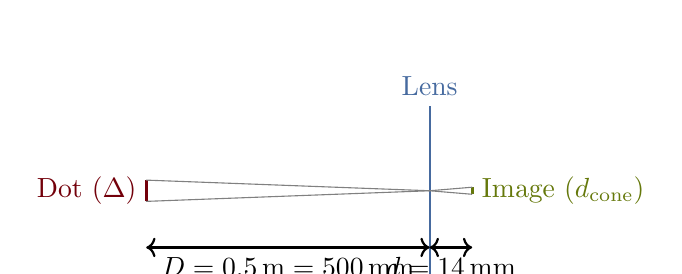
\begin{tikzpicture}[scale=0.9]
    % Lens
    \draw[thick, USC_Atlantic] (4, -1.2) -- (4, 1.2);
    \node[above, USC_Atlantic] at (4, 1.2) {Lens};

    % Object (dot)
    \draw[very thick, USC_Garnet] (0, -0.15) -- (0, 0.15);
    \node[left, USC_Garnet] at (0, 0) {Dot ($\Delta$)};

    % Image (on retina)
    \draw[very thick, USC_Honeycomb] (4.6, -0.05) -- (4.6, 0.05);
    \node[right, USC_Honeycomb] at (4.6, 0) {Image ($d_{\text{cone}}$)};

    % Rays
    \draw[thin, gray] (0, 0.15) -- (4, 0) -- (4.6, -0.05);
    \draw[thin, gray] (0, -0.15) -- (4, 0) -- (4.6, 0.05);

    % Distance labels
    \draw[<->, thick] (0, -0.8) -- (4, -0.8);
    \node[below] at (2, -0.8) {$D = 0.5\,\text{m} = 500\,\text{mm}$};
    \draw[<->, thick] (4, -0.8) -- (4.6, -0.8);
    \node[below] at (4.3, -0.8) {$d = 14\,\text{mm}$};
\end{tikzpicture}
\end{center}

By similar triangles:
\[
\frac{\Delta}{D} = \frac{d_{\text{cone}}}{d}
\]
\end{stepbox}

\begin{stepbox}[Step 3: Solve for Minimum Dot Diameter]
The smallest detectable image equals one cone diameter: $d_{\text{image}} = d_{\text{cone}} \approx 0.00258\,\text{mm}$.

\[
\Delta = D \cdot \frac{d_{\text{cone}}}{d} = 500 \cdot \frac{0.00258}{14} = \frac{1.29}{14} \approx 0.0922\,\text{mm}
\]
\end{stepbox}

\begin{resultsbox}
The diameter of the smallest printed dot that the eye can discern at a distance of 0.5\,m is:
\[
\boxed{\Delta \approx 0.0922\,\text{mm} \approx 92.2\,\mu\text{m}}
\]
\end{resultsbox}


% ============================================================================
% PROBLEM 2: Adjacency
% ============================================================================

\question{Problem 2: Adjacency of Image Subsets (25 pts)}\label{quest:2}

Consider the two image subsets $S_1$ and $S_2$ shown below. For $V = \{1\}$, determine whether these two subsets are (a) 4-adjacent, (b) 8-adjacent, or (c) m-adjacent.

\begin{center}
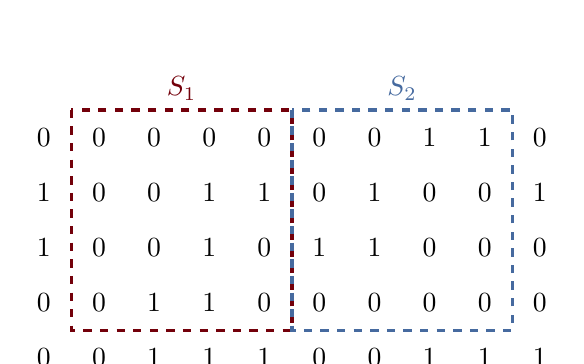
\begin{tikzpicture}[scale=0.7]
    % Row 0
    \node at (0,0) {0}; \node at (1,0) {0}; \node at (2,0) {0}; \node at (3,0) {0}; \node at (4,0) {0};
    \node at (5,0) {0}; \node at (6,0) {0}; \node at (7,0) {1}; \node at (8,0) {1}; \node at (9,0) {0};
    % Row 1
    \node at (0,-1) {1}; \node at (1,-1) {0}; \node at (2,-1) {0}; \node at (3,-1) {1}; \node at (4,-1) {1};
    \node at (5,-1) {0}; \node at (6,-1) {1}; \node at (7,-1) {0}; \node at (8,-1) {0}; \node at (9,-1) {1};
    % Row 2
    \node at (0,-2) {1}; \node at (1,-2) {0}; \node at (2,-2) {0}; \node at (3,-2) {1}; \node at (4,-2) {0};
    \node at (5,-2) {1}; \node at (6,-2) {1}; \node at (7,-2) {0}; \node at (8,-2) {0}; \node at (9,-2) {0};
    % Row 3
    \node at (0,-3) {0}; \node at (1,-3) {0}; \node at (2,-3) {1}; \node at (3,-3) {1}; \node at (4,-3) {0};
    \node at (5,-3) {0}; \node at (6,-3) {0}; \node at (7,-3) {0}; \node at (8,-3) {0}; \node at (9,-3) {0};
    % Row 4 (outside subsets)
    \node at (0,-4) {0}; \node at (1,-4) {0}; \node at (2,-4) {1}; \node at (3,-4) {1}; \node at (4,-4) {1};
    \node at (5,-4) {0}; \node at (6,-4) {0}; \node at (7,-4) {1}; \node at (8,-4) {1}; \node at (9,-4) {1};

    % S1 boundary (cols 1-4, rows 0-3)
    \draw[dashed, very thick, USC_Garnet] (0.5, 0.5) rectangle (4.5, -3.5);
    \node[above, USC_Garnet, font=\bfseries] at (2.5, 0.5) {$S_1$};

    % S2 boundary (cols 5-8, rows 0-3)
    \draw[dashed, very thick, USC_Atlantic] (4.5, 0.5) rectangle (8.5, -3.5);
    \node[above, USC_Atlantic, font=\bfseries] at (6.5, 0.5) {$S_2$};
\end{tikzpicture}
\end{center}



% --- Problem 2 Solution ---

\begin{stepbox}[Step 1: Identify Pixels in V = \{1\} Near the Boundary]
The subsets share the boundary between columns 4 (rightmost of $S_1$) and 5 (leftmost of $S_2$).

\textbf{$S_1$ pixels with value 1:} $(3,1)$, $(4,1)$, $(3,2)$, $(2,3)$, $(3,3)$ \quad (using $(x,y)$ coordinates from the grid).

\textbf{$S_2$ pixels with value 1:} $(7,0)$, $(8,0)$, $(6,1)$, $(5,2)$, $(6,2)$.

The closest cross-boundary pair in $V$ is $p = (4,1) \in S_1$ and $q = (5,2) \in S_2$.
\end{stepbox}

\begin{stepbox}[Step 2: Test Each Adjacency Type]
\textbf{(a) 4-adjacency:} Two subsets are 4-adjacent if $\exists\, p \in S_1, q \in S_2$ with values in $V$ that are 4-neighbors (share an edge). The nearest pair is $(4,1)$ and $(5,2)$, which differ in \emph{both} coordinates --- they are \emph{not} 4-neighbors. No other cross-boundary pair of pixels in $V$ is closer.

$\Rightarrow$ \textbf{$S_1$ and $S_2$ are NOT 4-adjacent.}

\vspace{0.3cm}
\textbf{(b) 8-adjacency:} $(4,1)$ and $(5,2)$ differ by 1 in each coordinate, so they are diagonal (8-)neighbors. Both have value $1 \in V$.

$\Rightarrow$ \textbf{$S_1$ and $S_2$ ARE 8-adjacent.}

\vspace{0.3cm}
\textbf{(c) m-adjacency:} Two pixels $p, q$ are m-adjacent if they are 8-adjacent \emph{and} $N_4(p) \cap N_4(q) \cap V = \varnothing$ (no shared 4-neighbor has a value in $V$). The shared 4-neighbors of $(4,1)$ and $(5,2)$ are $(4,2)$ and $(5,1)$:
\[
(4,2) = 0 \notin V, \qquad (5,1) = 0 \notin V.
\]
Since the intersection is empty, the m-adjacency condition is satisfied.

$\Rightarrow$ \textbf{$S_1$ and $S_2$ ARE m-adjacent.}
\end{stepbox}

\begin{resultsbox}
For $V = \{1\}$:
\begin{enumerate}[label=(\alph*)]
    \item $S_1$ and $S_2$ are \textbf{not} 4-adjacent.
    \item $S_1$ and $S_2$ \textbf{are} 8-adjacent (via $(4,1) \leftrightarrow (5,2)$).
    \item $S_1$ and $S_2$ \textbf{are} m-adjacent (via $(4,1) \leftrightarrow (5,2)$, since $N_4(p) \cap N_4(q) \cap V = \varnothing$).
\end{enumerate}
\end{resultsbox}


% ============================================================================
% PROBLEM 3: Shortest Paths
% ============================================================================

\question{Problem 3: Shortest Paths (25 pts)}\label{quest:3}

Consider the image segment shown below.

\begin{enumerate}[label=(\alph*)]
    \item Let $V = \{0, 1\}$ and compute the lengths of the shortest 4-, 8-, and m-path between $p$ and $q$. If a particular path does not exist between these two points, explain why.
    \item Repeat for $V = \{1, 2\}$.
\end{enumerate}

\begin{center}
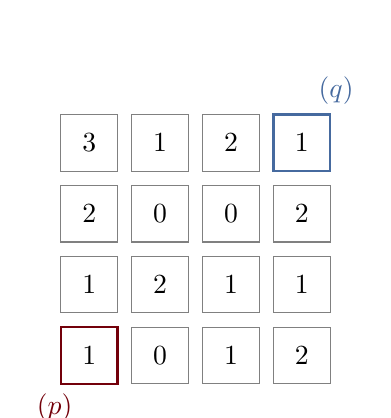
\begin{tikzpicture}[scale=0.9]
    % Row 0
    \draw[thin, gray] (-0.4,-0.4) rectangle (0.4,0.4); \node at (0,0) {3};
    \draw[thin, gray] (0.6,-0.4) rectangle (1.4,0.4); \node at (1,0) {1};
    \draw[thin, gray] (1.6,-0.4) rectangle (2.4,0.4); \node at (2,0) {2};
    \draw[thin, gray] (2.6,-0.4) rectangle (3.4,0.4); \node at (3,0) {1};
    % Row 1
    \draw[thin, gray] (-0.4,-1.4) rectangle (0.4,-0.6); \node at (0,-1) {2};
    \draw[thin, gray] (0.6,-1.4) rectangle (1.4,-0.6); \node at (1,-1) {0};
    \draw[thin, gray] (1.6,-1.4) rectangle (2.4,-0.6); \node at (2,-1) {0};
    \draw[thin, gray] (2.6,-1.4) rectangle (3.4,-0.6); \node at (3,-1) {2};
    % Row 2
    \draw[thin, gray] (-0.4,-2.4) rectangle (0.4,-1.6); \node at (0,-2) {1};
    \draw[thin, gray] (0.6,-2.4) rectangle (1.4,-1.6); \node at (1,-2) {2};
    \draw[thin, gray] (1.6,-2.4) rectangle (2.4,-1.6); \node at (2,-2) {1};
    \draw[thin, gray] (2.6,-2.4) rectangle (3.4,-1.6); \node at (3,-2) {1};
    % Row 3
    \draw[thin, gray] (-0.4,-3.4) rectangle (0.4,-2.6); \node at (0,-3) {1};
    \draw[thin, gray] (0.6,-3.4) rectangle (1.4,-2.6); \node at (1,-3) {0};
    \draw[thin, gray] (1.6,-3.4) rectangle (2.4,-2.6); \node at (2,-3) {1};
    \draw[thin, gray] (2.6,-3.4) rectangle (3.4,-2.6); \node at (3,-3) {2};

    % Mark p and q
    \node[below left, USC_Garnet, font=\bfseries] at (-0.1, -3.4) {$(p)$};
    \node[above right, USC_Atlantic, font=\bfseries] at (3.1, 0.4) {$(q)$};

    % Highlight p and q
    \draw[thick, USC_Garnet] (-0.4, -3.4) rectangle (0.4, -2.6);
    \draw[thick, USC_Atlantic] (2.6, -0.4) rectangle (3.4, 0.4);
\end{tikzpicture}
\end{center}


% --- Problem 3 Solution ---

\questionpart{Problem 3(a): $V = \{0, 1\}$}\label{quest:3a}

\begin{stepbox}[Step 1: Identify Pixels in V = \{0{,} 1\}]
Using $(c, r)$ (column, row) coordinates with the origin at the top-left:

\begin{center}
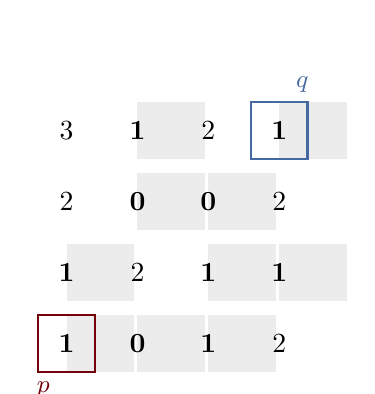
\begin{tikzpicture}[scale=0.9]
    % Row 0
    \fill[USC_Black10] (1,-0.4) rectangle (1.95,0.4);
    \fill[USC_Black10] (3,-0.4) rectangle (3.95,0.4);
    \node at (0,0) {3}; \node at (1,0) {\textbf{1}}; \node at (2,0) {2}; \node at (3,0) {\textbf{1}};
    % Row 1
    \fill[USC_Black10] (1,-1.4) rectangle (1.95,-0.6);
    \fill[USC_Black10] (2,-1.4) rectangle (2.95,-0.6);
    \node at (0,-1) {2}; \node at (1,-1) {\textbf{0}}; \node at (2,-1) {\textbf{0}}; \node at (3,-1) {2};
    % Row 2
    \fill[USC_Black10] (0,-2.4) rectangle (0.95,-1.6);
    \fill[USC_Black10] (2,-2.4) rectangle (2.95,-1.6);
    \fill[USC_Black10] (3,-2.4) rectangle (3.95,-1.6);
    \node at (0,-2) {\textbf{1}}; \node at (1,-2) {2}; \node at (2,-2) {\textbf{1}}; \node at (3,-2) {\textbf{1}};
    % Row 3
    \fill[USC_Black10] (0,-3.4) rectangle (0.95,-2.6);
    \fill[USC_Black10] (1,-3.4) rectangle (1.95,-2.6);
    \fill[USC_Black10] (2,-3.4) rectangle (2.95,-2.6);
    \node at (0,-3) {\textbf{1}}; \node at (1,-3) {\textbf{0}}; \node at (2,-3) {\textbf{1}}; \node at (3,-3) {2};

    % p and q
    \draw[thick, USC_Garnet] (-0.4,-3.4) rectangle (0.4,-2.6);
    \draw[thick, USC_Atlantic] (2.6,-0.4) rectangle (3.4,0.4);
    \node[below left, USC_Garnet, font=\bfseries\small] at (-0.1,-3.4) {$p$};
    \node[above right, USC_Atlantic, font=\bfseries\small] at (3.1,0.4) {$q$};
\end{tikzpicture}
\end{center}
Shaded cells have values in $V$. $p = (0,3) = 1 \in V$, $q = (3,0) = 1 \in V$.
\end{stepbox}

\begin{stepbox}[Step 2: Shortest 4-Path]
For a 4-path, each step moves to a horizontal or vertical neighbor in $V$.

Pixel $q = (3,0)$ has 4-neighbors $(2,0) = 2 \notin V$ and $(3,1) = 2 \notin V$. Therefore $q$ is \textbf{isolated} in $V$ under 4-connectivity.

$\Rightarrow$ \textbf{No 4-path exists.}
\end{stepbox}

\begin{stepbox}[Step 3: Shortest 8-Path]
For an 8-path, each step moves to any of the 8 surrounding neighbors in $V$.

$q = (3,0)$ has 8-neighbor $(2,1) = 0 \in V$, so $q$ is reachable. One shortest path:
\[
(0,3) \to (0,2) \to (1,1) \to (2,1) \to (3,0)
\]
\begin{itemize}
    \item $(0,3) \to (0,2)$: 4-adj, values $1, 1 \in V$ \checkmark
    \item $(0,2) \to (1,1)$: diagonal, values $1, 0 \in V$ \checkmark
    \item $(1,1) \to (2,1)$: 4-adj, values $0, 0 \in V$ \checkmark
    \item $(2,1) \to (3,0)$: diagonal, values $0, 1 \in V$ \checkmark
\end{itemize}
Length = \textbf{4}. No shorter path exists (minimum diagonal steps $\geq 3$, and no 3-step path can be constructed).
\end{stepbox}

\begin{stepbox}[Step 4: Shortest m-Path]
For m-adjacency, a diagonal step is allowed only if the two shared 4-neighbors are not both in $V$.

Checking each diagonal in the 8-path above:
\begin{itemize}
    \item $(0,2) \to (1,1)$: shared 4-neighbors are $(0,1) = 2 \notin V$ and $(1,2) = 2 \notin V$. $\checkmark$
    \item $(2,1) \to (3,0)$: shared 4-neighbors are $(2,0) = 2 \notin V$ and $(3,1) = 2 \notin V$. $\checkmark$
\end{itemize}
All diagonal steps satisfy the m-adjacency condition, so the same path is valid.

Length = \textbf{4}.
\end{stepbox}

\begin{resultsbox}
For $V = \{0,1\}$:
\begin{itemize}
    \item \textbf{Shortest 4-path:} Does not exist ($q$ is 4-isolated in $V$).
    \item \textbf{Shortest 8-path:} Length \textbf{4}: $(0,3) \to (0,2) \to (1,1) \to (2,1) \to (3,0)$.
    \item \textbf{Shortest m-path:} Length \textbf{4}: same path (all diagonals satisfy m-adjacency).
\end{itemize}
\end{resultsbox}

\questionpart{Problem 3(b): $V = \{1, 2\}$}\label{quest:3b}

\begin{stepbox}[Step 1: Identify Pixels in V = \{1{,} 2\}]
\begin{center}
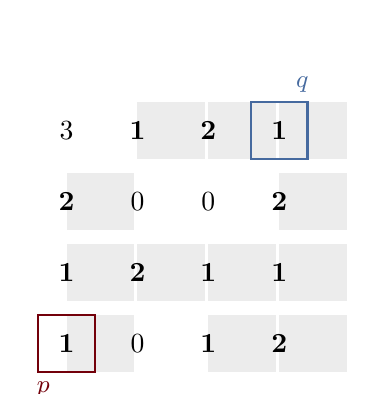
\begin{tikzpicture}[scale=0.9]
    % Row 0
    \fill[USC_Black10] (1,-0.4) rectangle (1.95,0.4);
    \fill[USC_Black10] (2,-0.4) rectangle (2.95,0.4);
    \fill[USC_Black10] (3,-0.4) rectangle (3.95,0.4);
    \node at (0,0) {3}; \node at (1,0) {\textbf{1}}; \node at (2,0) {\textbf{2}}; \node at (3,0) {\textbf{1}};
    % Row 1
    \fill[USC_Black10] (0,-1.4) rectangle (0.95,-0.6);
    \fill[USC_Black10] (3,-1.4) rectangle (3.95,-0.6);
    \node at (0,-1) {\textbf{2}}; \node at (1,-1) {0}; \node at (2,-1) {0}; \node at (3,-1) {\textbf{2}};
    % Row 2
    \fill[USC_Black10] (0,-2.4) rectangle (0.95,-1.6);
    \fill[USC_Black10] (1,-2.4) rectangle (1.95,-1.6);
    \fill[USC_Black10] (2,-2.4) rectangle (2.95,-1.6);
    \fill[USC_Black10] (3,-2.4) rectangle (3.95,-1.6);
    \node at (0,-2) {\textbf{1}}; \node at (1,-2) {\textbf{2}}; \node at (2,-2) {\textbf{1}}; \node at (3,-2) {\textbf{1}};
    % Row 3
    \fill[USC_Black10] (0,-3.4) rectangle (0.95,-2.6);
    \fill[USC_Black10] (2,-3.4) rectangle (2.95,-2.6);
    \fill[USC_Black10] (3,-3.4) rectangle (3.95,-2.6);
    \node at (0,-3) {\textbf{1}}; \node at (1,-3) {0}; \node at (2,-3) {\textbf{1}}; \node at (3,-3) {\textbf{2}};

    % p and q
    \draw[thick, USC_Garnet] (-0.4,-3.4) rectangle (0.4,-2.6);
    \draw[thick, USC_Atlantic] (2.6,-0.4) rectangle (3.4,0.4);
    \node[below left, USC_Garnet, font=\bfseries\small] at (-0.1,-3.4) {$p$};
    \node[above right, USC_Atlantic, font=\bfseries\small] at (3.1,0.4) {$q$};
\end{tikzpicture}
\end{center}
Shaded cells have values in $V$. Both $p$ and $q$ are now well-connected.
\end{stepbox}

\begin{stepbox}[Step 2: Shortest 4-Path]
A valid 4-path:
\[
(0,3) \to (0,2) \to (1,2) \to (2,2) \to (3,2) \to (3,1) \to (3,0)
\]
Length = \textbf{6}. Every step is a 4-neighbor in $V$. No shorter 4-path exists because the middle rows have 0-valued pixels at $(1,1)$ and $(2,1)$ that block more direct routes.
\end{stepbox}

\begin{stepbox}[Step 3: Shortest 8-Path]
Using diagonal moves:
\[
(0,3) \to (1,2) \to (2,2) \to (3,1) \to (3,0)
\]
\begin{itemize}
    \item $(0,3) \to (1,2)$: diagonal, values $1, 2 \in V$ \checkmark
    \item $(1,2) \to (2,2)$: 4-adj, values $2, 1 \in V$ \checkmark
    \item $(2,2) \to (3,1)$: diagonal, values $1, 2 \in V$ \checkmark
    \item $(3,1) \to (3,0)$: 4-adj, values $2, 1 \in V$ \checkmark
\end{itemize}
Length = \textbf{4}. No 3-step path exists.
\end{stepbox}

\begin{stepbox}[Step 4: Shortest m-Path]
Check each diagonal step:
\begin{itemize}
    \item $(0,3) \to (1,2)$: shared 4-neighbors are $(0,2) = 1 \in V$ and $(1,3) = 0 \notin V$. Since $(0,2) \in V$, this diagonal is \textbf{not} m-adjacent.
    \item $(2,2) \to (3,1)$: shared 4-neighbors are $(2,1) = 0 \notin V$ and $(3,2) = 1 \in V$. Since $(3,2) \in V$, this diagonal is \textbf{not} m-adjacent.
\end{itemize}
Both diagonals fail. We must replace each with two 4-adjacent steps. The shortest m-path:
\[
(0,3) \to (0,2) \to (1,2) \to (2,2) \to (3,2) \to (3,1) \to (3,0)
\]
Length = \textbf{6}.
\end{stepbox}

\begin{resultsbox}
For $V = \{1,2\}$:
\begin{itemize}
    \item \textbf{Shortest 4-path:} Length \textbf{6}: $(0,3) \to (0,2) \to (1,2) \to (2,2) \to (3,2) \to (3,1) \to (3,0)$.
    \item \textbf{Shortest 8-path:} Length \textbf{4}: $(0,3) \to (1,2) \to (2,2) \to (3,1) \to (3,0)$.
    \item \textbf{Shortest m-path:} Length \textbf{6}: $(0,3) \to (0,2) \to (1,2) \to (2,2) \to (3,2) \to (3,1) \to (3,0)$.
\end{itemize}
\end{resultsbox}


% ============================================================================
% PROBLEM 4: Set Expressions
% ============================================================================

\question{Problem 4: Set Expressions (25 pts)}\label{quest:4}

Give expressions for the sets shown shaded in the following figure in terms of sets $A$, $B$, and $C$. The shaded areas in each figure constitute one set, so give one expression for each of the three figures.

% --- Individual shapes A, B, C ---
\begin{center}
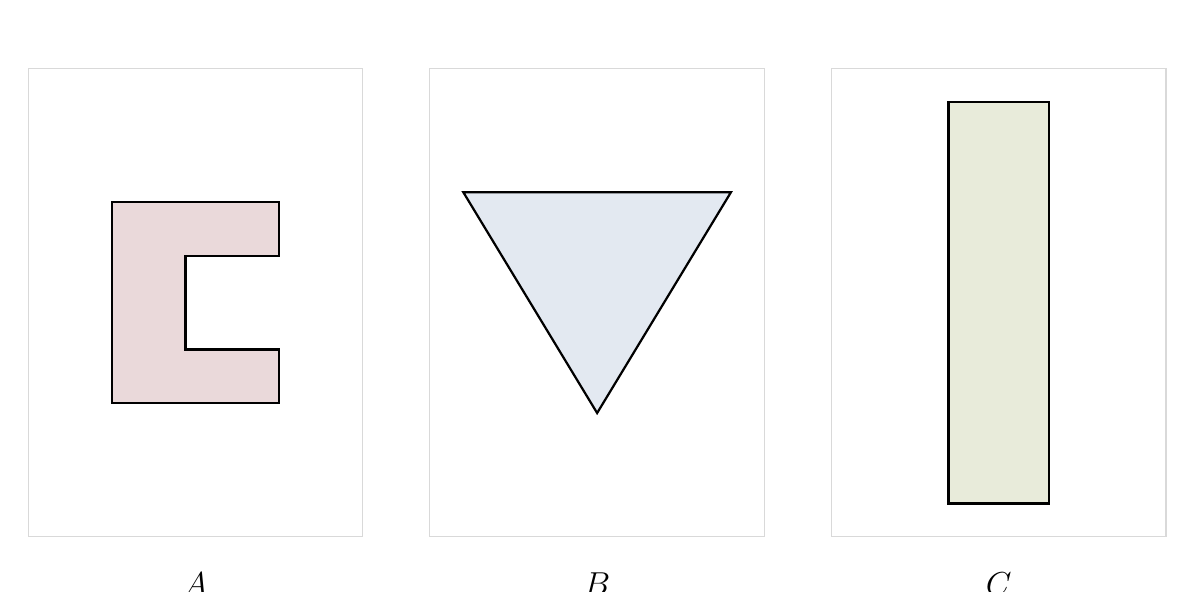
\begin{tikzpicture}[scale=0.85]

    % All columns are 5 units wide, centered at x = 2.5, 8.5, 14.5

    % === Shape A (width 2.5, height 3) -> center at (2.5, 3) ===
    \begin{scope}[shift={(0,0)}]
        \draw[gray!30, thin] (0,-0.5) rectangle (5,6.5);
        \fill[USC_Garnet!15] (1.25,1.5) -- (3.75,1.5) -- (3.75,2.3) -- (2.35,2.3) -- (2.35,3.7) -- (3.75,3.7) -- (3.75,4.5) -- (1.25,4.5) -- cycle;
        \draw[thick] (1.25,1.5) -- (3.75,1.5) -- (3.75,2.3) -- (2.35,2.3) -- (2.35,3.7) -- (3.75,3.7) -- (3.75,4.5) -- (1.25,4.5) -- cycle;
        \node[font=\large\bfseries] at (2.5, -1.2) {$A$};
    \end{scope}

    % === Shape B (width 4, height 3.3) -> center at (8.5, 3) ===
    \begin{scope}[shift={(6,0)}]
        \draw[gray!30, thin] (0,-0.5) rectangle (5,6.5);
        \fill[USC_Atlantic!15] (0.5,4.65) -- (4.5,4.65) -- (2.5,1.35) -- cycle;
        \draw[thick] (0.5,4.65) -- (4.5,4.65) -- (2.5,1.35) -- cycle;
        \node[font=\large\bfseries] at (2.5, -1.2) {$B$};
    \end{scope}

    % === Shape C (width 1.5, height 6) -> center at (14.5, 3) ===
    \begin{scope}[shift={(12,0)}]
        \draw[gray!30, thin] (0,-0.5) rectangle (5,6.5);
        \fill[USC_Honeycomb!15] (1.75,0) -- (3.25,0) -- (3.25,6) -- (1.75,6) -- cycle;
        \draw[thick] (1.75,0) -- (3.25,0) -- (3.25,6) -- (1.75,6) -- cycle;
        \node[font=\large\bfseries] at (2.5, -1.2) {$C$};
    \end{scope}

\end{tikzpicture}
\end{center}

% Pre-computed world coordinates:
% A: (0,3) -- (2.5,3) -- (2.5,3.8) -- (1.1,3.8) -- (1.1,5.2) -- (2.5,5.2) -- (2.5,6) -- (0,6) -- cycle
% B: (-0.99,3.96) -- (3.41,3.96) -- (1.21,0.33) -- cycle
% C: (2,0.2) -- (3.5,0.2) -- (3.5,6.2) -- (2,6.2) -- cycle

% Macros for shape paths
\newcommand{\pathA}{(0,3) -- (2.5,3) -- (2.5,3.8) -- (1.1,3.8) -- (1.1,5.2) -- (2.5,5.2) -- (2.5,6) -- (0,6) -- cycle}
\newcommand{\pathB}{(-0.99,3.96) -- (3.41,3.96) -- (1.21,0.33) -- cycle}
\newcommand{\pathC}{(2,0.2) -- (3.5,0.2) -- (3.5,6.2) -- (2,6.2) -- cycle}

\vspace{0.5cm}
\hrule
\vspace{0.5cm}

% --- Three shaded figures ---
\begin{center}
\begin{tikzpicture}[scale=0.8]

    % ============================
    % FIGURE (i): A ∩ B ∩ C
    % ============================
    \begin{scope}[shift={(0,0)}]
        \begin{scope}
            \clip \pathA;
            \clip \pathB;
            \clip \pathC;
            \fill[gray!40] (-2,-1) rectangle (5,7);
        \end{scope}
        \draw[thick] \pathA;
        \draw[thick] \pathB;
        \draw[thick] \pathC;
        \node[below] at (1.5, -0.5) {(i)};
    \end{scope}

    % ============================
    % FIGURE (ii): (A∩B) ∪ (B∩C) ∪ (A∩C)
    % ============================
    \begin{scope}[shift={(8,0)}]
        % Shade A ∩ B
        \begin{scope}
            \clip \pathA;
            \clip \pathB;
            \fill[gray!40] (-2,-1) rectangle (5,7);
        \end{scope}
        % Shade B ∩ C
        \begin{scope}
            \clip \pathB;
            \clip \pathC;
            \fill[gray!40] (-2,-1) rectangle (5,7);
        \end{scope}
        % Shade A ∩ C
        \begin{scope}
            \clip \pathA;
            \clip \pathC;
            \fill[gray!40] (-2,-1) rectangle (5,7);
        \end{scope}
        \draw[thick] \pathA;
        \draw[thick] \pathB;
        \draw[thick] \pathC;
        \node[below] at (1.5, -0.5) {(ii)};
    \end{scope}

    % ============================
    % FIGURE (iii): (B ∩ A^c ∩ C^c) ∪ (A ∩ C ∩ B^c)
    % ============================
    \begin{scope}[shift={(16,0)}]
        % Shade B
        \begin{scope}
            \clip \pathB;
            \fill[gray!40] (-2,-1) rectangle (5,7);
        \end{scope}
        % Remove B ∩ A
        \begin{scope}
            \clip \pathB;
            \clip \pathA;
            \fill[white] (-2,-1) rectangle (5,7);
        \end{scope}
        % Remove B ∩ C
        \begin{scope}
            \clip \pathB;
            \clip \pathC;
            \fill[white] (-2,-1) rectangle (5,7);
        \end{scope}
        % Shade A ∩ C
        \begin{scope}
            \clip \pathA;
            \clip \pathC;
            \fill[gray!40] (-2,-1) rectangle (5,7);
        \end{scope}
        % Remove A ∩ C ∩ B
        \begin{scope}
            \clip \pathA;
            \clip \pathC;
            \clip \pathB;
            \fill[white] (-2,-1) rectangle (5,7);
        \end{scope}
        \draw[thick] \pathA;
        \draw[thick] \pathB;
        \draw[thick] \pathC;
        \node[below] at (1.5, -0.5) {(iii)};
    \end{scope}

\end{tikzpicture}
\end{center}


% --- Problem 4 Solution ---

\begin{stepbox}[Step 1: Analyze Each Shaded Region]
We identify the shaded areas in each figure by examining which combinations of sets $A$, $B$, and $C$ overlap:

\textbf{Figure (i):} The shaded region is the area where \emph{all three} sets overlap simultaneously. This is the triple intersection.

\textbf{Figure (ii):} The shaded region covers every area where \emph{at least two} of the three sets overlap. This includes the pairwise intersections $A \cap B$, $B \cap C$, and $A \cap C$ (and their common triple intersection).

\textbf{Figure (iii):} Two disjoint shaded regions appear: the part of $B$ that lies outside both $A$ and $C$, and the part of $A \cap C$ that lies outside $B$.
\end{stepbox}

\begin{resultsbox}
\begin{enumerate}[label=(\roman*)]
    \item $A \cap B \cap C$
    \item $(A \cap B) \cup (B \cap C) \cup (A \cap C)$
    \item $(B \cap A^c \cap C^c) \cup (A \cap C \cap B^c)$
\end{enumerate}
\end{resultsbox}


% ============================================================================
% END OF DOCUMENT
% ============================================================================

\end{document}
